\section{Data}
In this chapter we answer to question EQ1, asking to find the biggest LoRa SF for
having a success rate of at least 70\% in a LoRaWAN Network with the following parameters:
\begin{itemize}
\item Carrier frequency: $CF = 868 MHz$
\item Bandwidth: $BW = 125 kHz$
\item Number of gateways: $N_{G} = 1$
\item Number of sensor nodes: $N_{S} = 50$
\item Intensity of Poisson process: $\lambda = 1 \text{ packet/minute}$
\item Success rate: $SR \geq 0.7$
\end{itemize}

We compute the payload size based on the last two digits of the leader's person code (XY), according to the formula:
\begin{equation}
L = 3 + XY \text{ Bytes}
\end{equation}
Our leader's person code is 10773593, so the payload size is:
\begin{equation}
L = 3 + 93 = 96 \text{ Bytes}
\end{equation}

\section{Maximum Spreading Factor calculation}
Since LoRaWAN uses an ALOHA-like procedure to handle channel access and
retransmissions, we compute the success rate, SR, as the ALOHA success rate:
\begin{equation}
SR = S / G = e^{-2 G} = e^{-2 N \lambda t}
\end{equation}

Thanks to this formula, we can compute the maximum airtime to have a success rate greater than 70\%.
\begin{equation}
SR \geq 0.7
\end{equation}
\begin{equation}
e^{-2 N \lambda t} \geq 0.7
\end{equation}
By applying the natural logarithm, we get:
\begin{equation}
-2 N \lambda t \geq ln(0.7)
\end{equation}
\begin{equation}
t \leq \frac{-ln(0.7)}{2 N \lambda} = \frac{-ln(0.7)}{2 \cdot 50 \cdot \frac{1}{60 \cdot 10^3 \text{ ms}}} = 214.005 \text{ ms}
\end{equation}

We now use the API offered by The Things Network at {\color{blue}\url{https://www.thethingsnetwork.org/airtime-calculator}} to find the highest SF that guarantees an airtime smaller than the value we found. We use payload size of 96 Bytes, as computed before, region EU868 and bandwidth 125 kHz. The API says that the maximum payload size for EU868 with SF from 10 to 12 is 51 Bytes; this means that we can evaluate SF values starting from 9 and lowering the SF until we find an airtime smaller than 214.005 ms.
The values of airtime corresponding to the SF are report in the following table.

\begin{table}[H]
\centering 
\begin{tabular}{| c | c |}
	\hline 
	\rowcolor{bluepoli!40}
	\textbf{Spreading Factor} & \textbf{Airtime}\T\B \\
	\hline 
	SF9 & 594.9 ms \T\B\\
	SF8  & 328.2 ms \T\B\\
	SF7 & 184.6 ms \T\B\\
	\hline
\end{tabular}
\\[10pt]
\caption{Airtime based on SF}
\end{table}

The only value of SF that leads to an airtime smaller than 214.005 ms and a success rate greater than 70\% is SF7.

\begin{figure}[H]
    \centering
    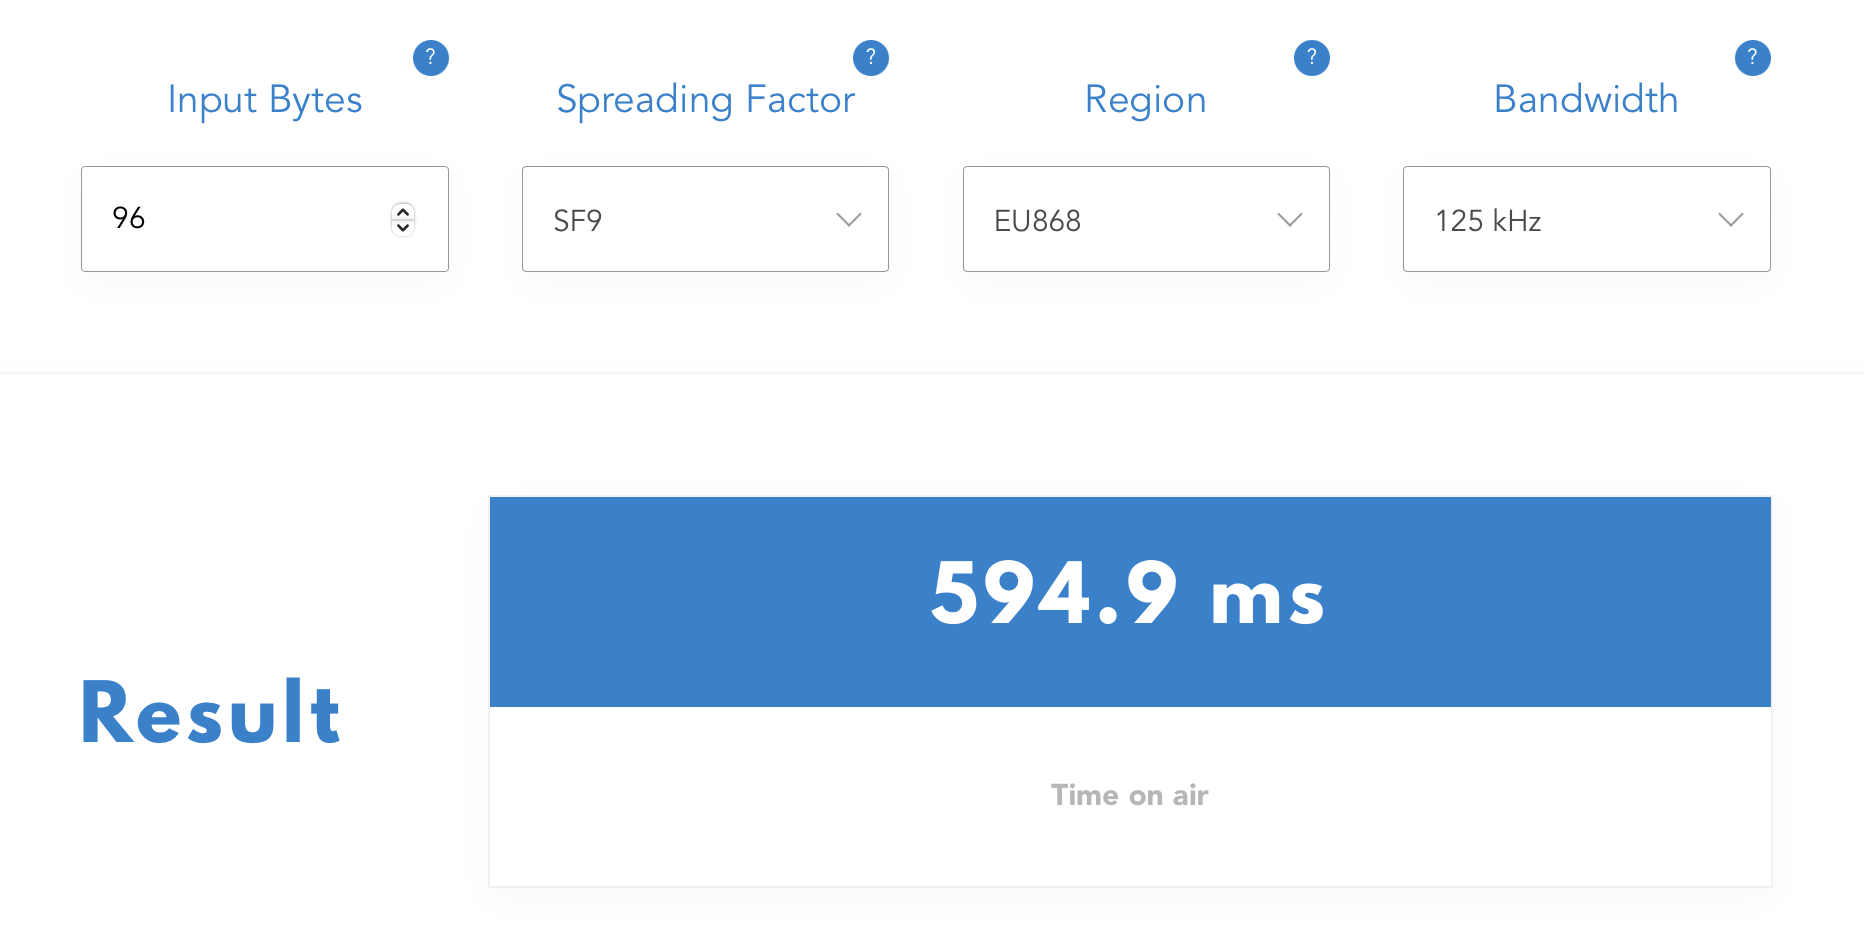
\includegraphics[width=0.6\linewidth, height=0.5\textheight, keepaspectratio]{sf9.png}
    \caption{Airtime with SF9}
\end{figure}

\begin{figure}[H]
    \centering
    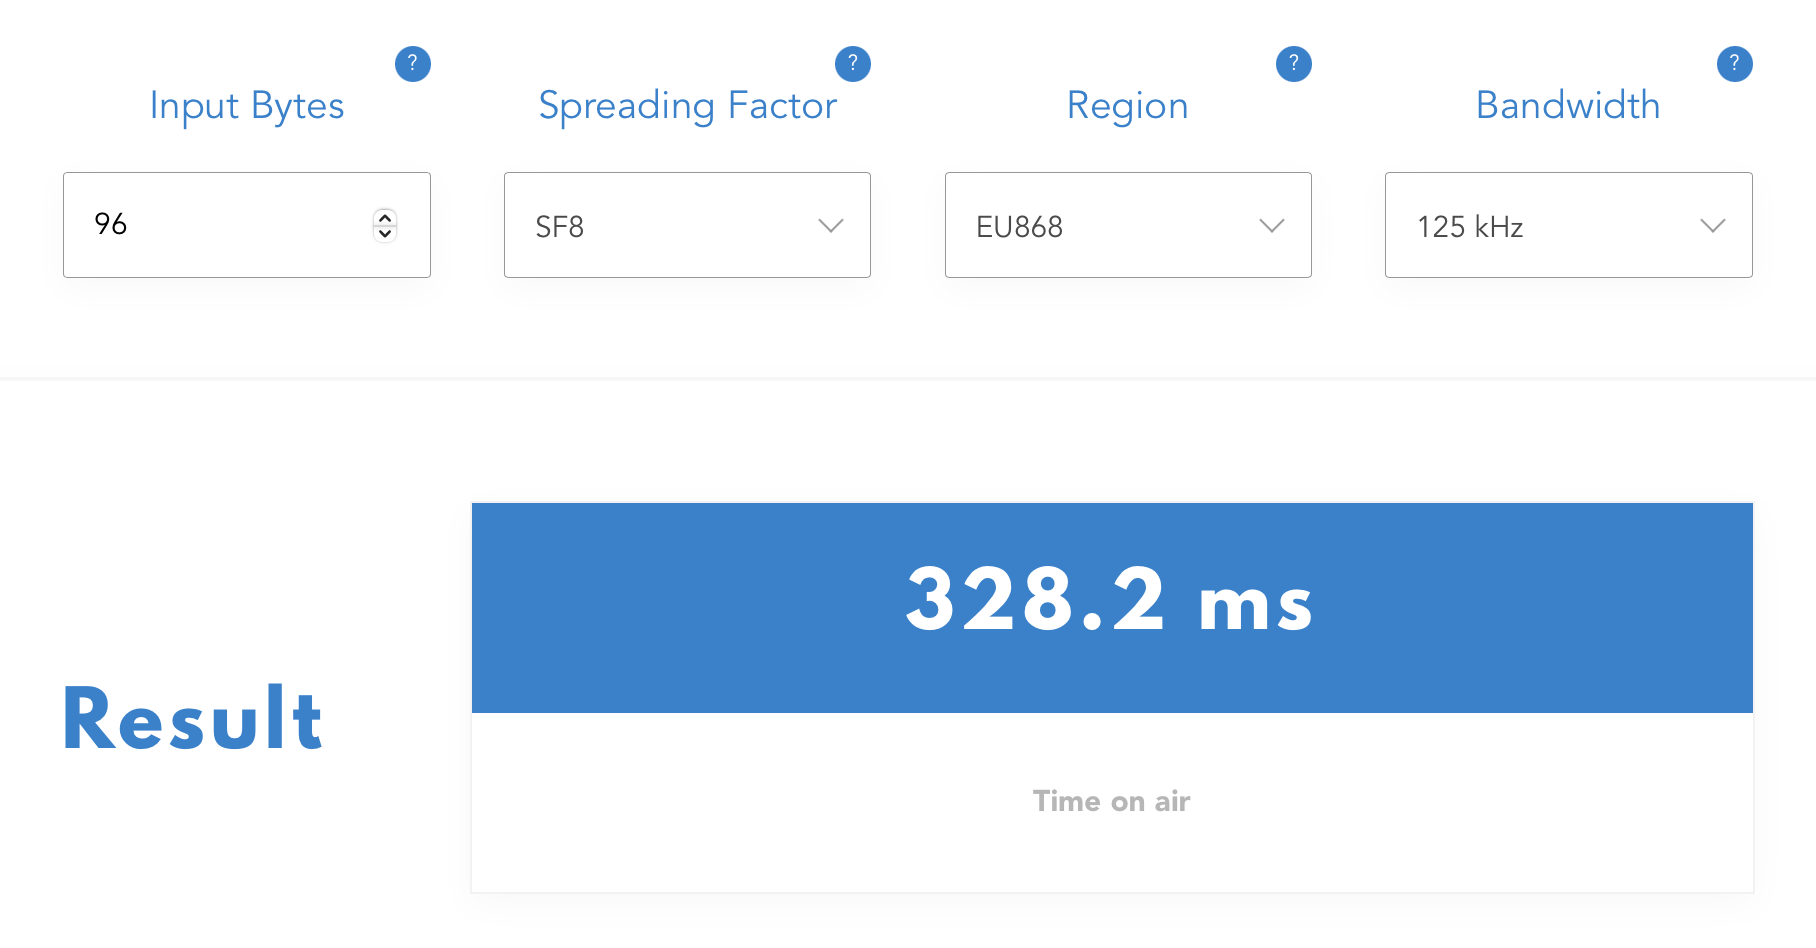
\includegraphics[width=0.6\linewidth, height=0.5\textheight, keepaspectratio]{sf8.png}
    \caption{Airtime with SF8}
\end{figure}

\begin{figure}[H]
    \centering
    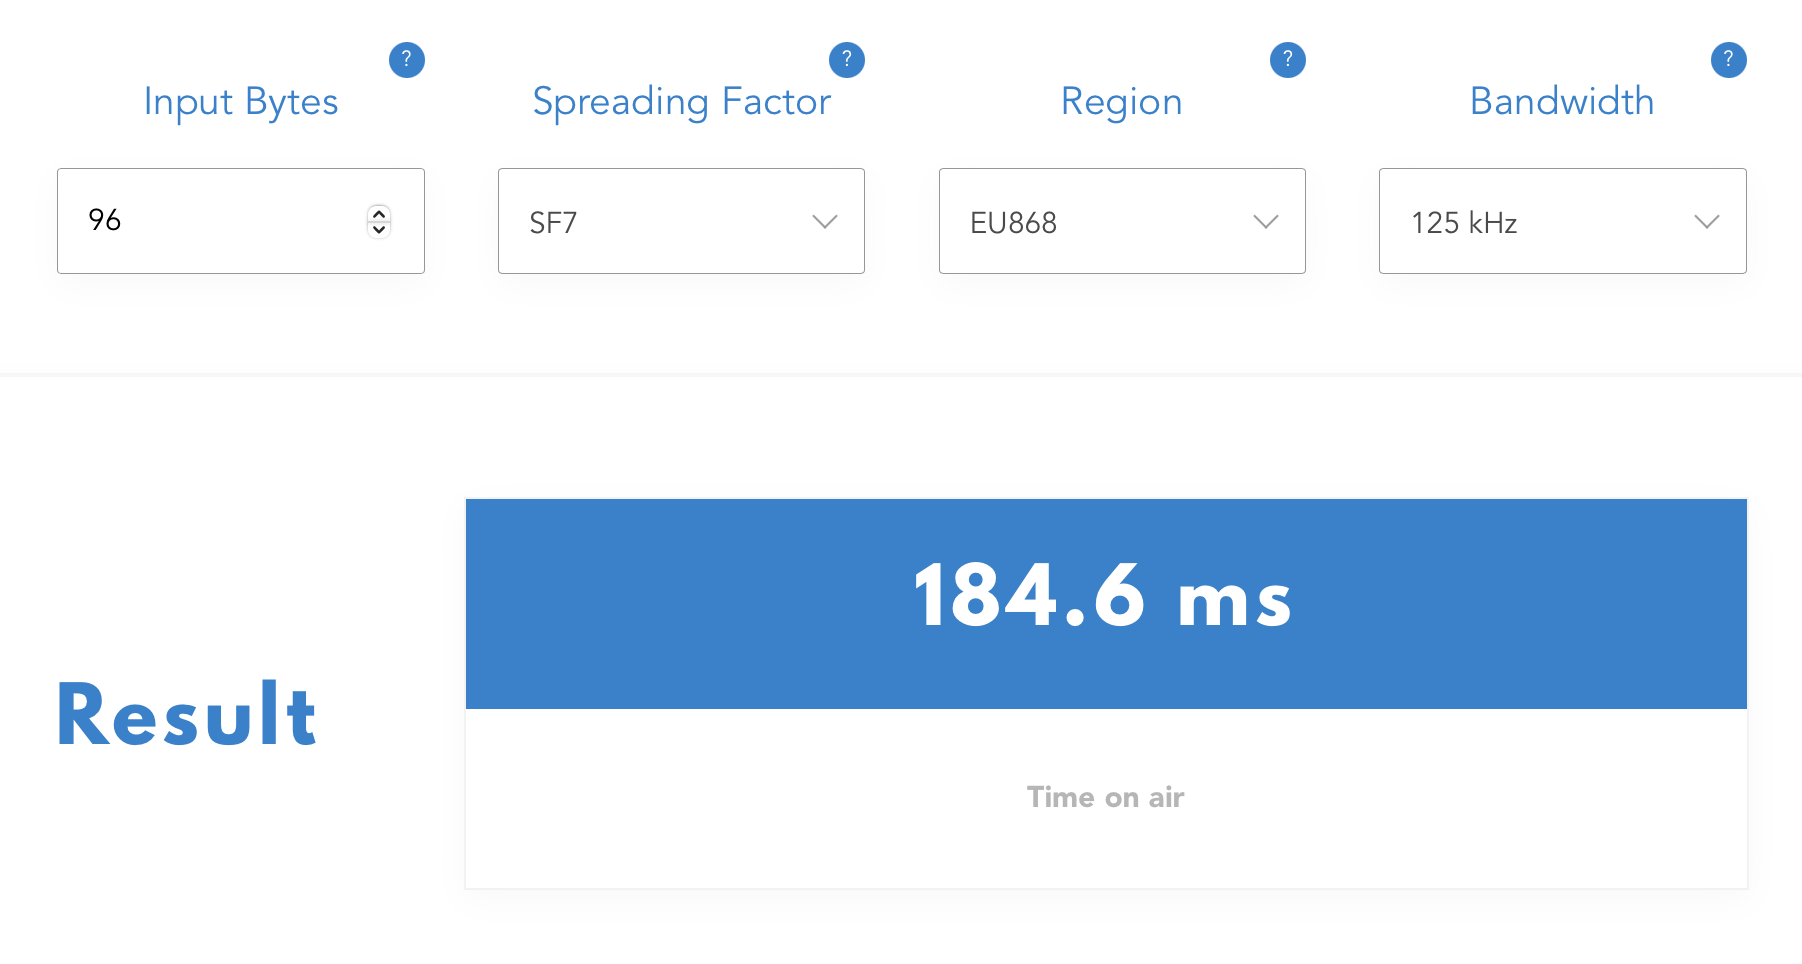
\includegraphics[width=0.6\linewidth, height=0.5\textheight, keepaspectratio]{sf7.png}
    \caption{Airtime with SF7}
\end{figure}




